% !TEX root = ../main.tex
\label{section:theoreticalBackground}
\section{Theoretical Background}
In this section, we begin with introducing the general problem of optimisation. This is followed by the formulation of constrained optimisation problems, for which we give a more detailed description of different solving approaches. In particular, we focus on the Penalty Method and the Augmented Lagrangian Method.
\subsection{Optimisation problems}
\label{ssec:opt_prob}
Optimisation problems are subject to mathematicians and scientists in finding the best solution for a given problem. Formally, an optimisation problem can be described as minimising an objective function $f$, that is, 
\begin{equation}
\argmin_{x \in \mathbb{R}^n} f(x),
\end{equation}
where $f\colon \mathbb{R}^n\to \mathbb{R}$ is the smooth function to be minimised and $n \in \mathbb{N}$ is the input dimension. In general, optimisation problems can be divided into several categories depending on properties of the objective function $f$. In the following, we briefly describe the most important categories of unconstrained optimisation problems.
\begin{figure}[H]
	\centering
	\begin{subfigure}{.32\textwidth}
		\centering
		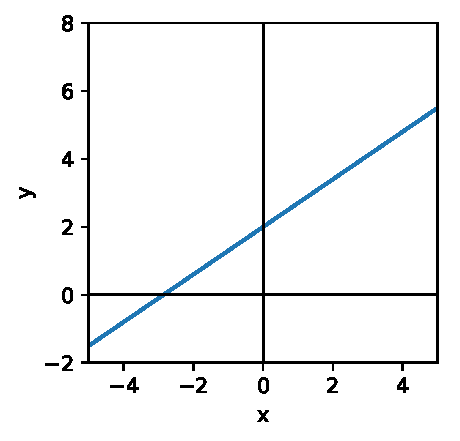
\includegraphics[width=\linewidth]{fn_lin}
		\caption{$f(x) = 0.7x + 2$}
		\label{fn_a}
	\end{subfigure}%
	\begin{subfigure}{.32\textwidth}
	\centering
	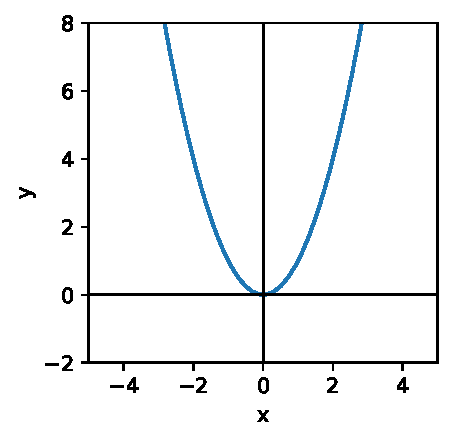
\includegraphics[width=\linewidth]{fn_con}
		\caption{$f(x) = x^2$}
		\label{fn_b}
\end{subfigure}%
	\begin{subfigure}{.32\textwidth}
	\centering
	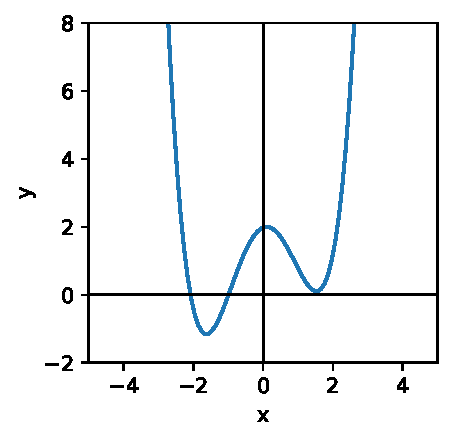
\includegraphics[width=\linewidth]{fn_any}
		\caption{$f(x) = 0.4x^4 - 2(x-0.1)^2 + 2$}
		\label{fn_c}
\end{subfigure}%
	\caption{Example for a strictly monotonic function (\ref{fn_a}), a strictly convex function (\ref{fn_b}) and a function with different local and global minima (\ref{fn_c}).}
	\label{fig:mu_lambda_alm_dyn}
\end{figure}
\subsubsection{Strictly monotonic functions}
The first category of minimisation problems are the ones with a strictly increasing (resp. decreasing) objective function $f$. Formally, for $n = 1$, this is the case if $\forall a, b \in \mathbb{R}: a > b \Rightarrow f(a) < f(b)$ (resp. $f(a) > f(b)$). All linear functions of the form $f(x) = mx + t$ with $m \neq 0$ are strictly monotonic. An example for a linear and strictly monotonic function is shown in Figure \ref{fn_a}. However, these functions do not have any global minima in an open domain and the optimisation problem therefore has no solution. For bounded domain spaces, the global minimum is located on the boundary of the domain.
\subsubsection{Strictly convex functions}
In addition to strictly monotonic functions, we want to introduce optimisation problems with strictly convex objective functions. Formally, a function is strictly convex if it satisfies the following condition:
\[ \forall a, b \in \mathbb{R}^d, \forall \lambda \in (0, 1): \qquad f(\lambda a + (1 - \lambda) b) < \lambda f(a) + (1- \lambda)f(b) \]
An example for a strictly convex function is $f(x) = x^2$, as depicted in Figure \ref{fn_b}. Optimisation problems with a strictly convex objective functions are rather easy to solve, since there exists only one local minimum, which is also the global minimum.
\subsubsection{Functions with different local and global optima}
The third category we present contains optimisation problems whose functions have multiple local minima and at least one global minimum. As a consequence, an obtained local minimum is not necessarily a global optimum and therefore it might not be the solution to the problem. To give an example, the function depicted in Figure \ref{fn_c} has a global minimum at $x \approx -1.6$, but also a local minimum at $x \approx 1.6$. For this reason, solving optimisation problems of this category is usually difficult.\\
\subsubsection{Solving methods}
In general, it is desirable to obtain a solution for an unconstrained optimisation problem analytically, because one can rely on finding an exact global optimum when using analytical methods. For strictly convex functions, one can find the minimum by searching for the root of the derivative of the objective function, since only the single existing local minimum has a gradient of zero. For example, one can easily find the minimum of $f(x) = x^2$ by calculating the root of $f'(x) = 2x$, which is $x = 0$. For more complex functions however, obtaining a solution of the optimisation problem is analytically not feasible. For this reason, such problems have to be solved using algorithms that find numeric solutions. The main approach of numeric optimisation algorithms is described by Nocedal et al. in \cite{NoceWrig06}. In general, numeric algorithms do not exploit analytical characteristics of the function, but instead only use properties of the objective function at a specific point, which includes e.g. the value of $f$ and its gradient. For this reason, the main approach of optimisation algorithms is to start at an initial guess $x_0$ and to iteratively calculate a following iterate $x_{k+1}$ with the use of information about $f$ at the previous iterates $x_0, x_1, ..., x_k$. With this procedure, such an algorithm generates a sequence of iterates $\{x_k\}_{k=0}^\infty$. Optimisation algorithms are usually designed to converge to a local minimum, but have no guarantee for approximating one of the global optima. The sequence is terminated either once a sufficiently good approximation of the solution is found, or when the sequence converges, meaning that the distances between the last iterates are extremely small. If no solution exists, which is the case when no point minimises the objective function, the algorithm might not terminate, since for any iterate a point with a smaller objective value can be found. The core of the algorithms is the way they use information about $f$ at the points $x_0, x_1, ..., x_k$ to compute $x_{k+1}$. \\
\indent Nocedal et al. introduce two categories of optimisation algorithms: Line search and trust region strategies. The former first determines a line on which the next iterate is located, and then tries to find a point $x_{k+1}$ such that $f(x_{k+1}) < f(x_k)$. Finding such an iterate is much simpler than the original minimisation problem, since a search only has to be performed along one dimension. A commonly used approach is the steepest descent method, where the direction is chosen to be the negative gradient, since it offers the locally steepest decent. Another important approach is to choose the Newton direction, which is calculated by finding a vector $p$ minimising the second-order Taylor series approximation to $f(x_k + p)$. Line search methods also include quasi-Newton methods and conjugate gradient methods.\\ 
\indent In contrast to line search methods, trust region strategies approximate the behaviour of the objective function $f$ inside a trust region $T$ around $x_k$ using a simpler model function $m_k$. The model function is often computed using the first terms of the Taylor expansion, that is, \[m_k(x_k + p) = f(x_k) + p^T\Delta f(x_k) + \frac{1}{2}p^T\Delta^2 f(x_k) p \text{, \indent where } x_k + p \in T.\] Since the Hessian $\Delta^2 f(x_k)$ of the objective function can be hard to compute or not accessable, it can also be replaced by an approximation, which is for example calculated using the SR1 or BFGS formula \cite{NoceWrig06}. The iterate $x_{k+1}$ is then set to be the solution of the simpler problem $x_{k+1} = \underset{x \in T}{\argmin }  \,\,m_k(x)$. Examples for trust region methods are the Dogleg method and Seihaug's approach \cite{NoceWrig06}.

\subsection{Constrained optimisation problems}
\label{ssec:copt_prob}
A constrained optimisation problem is an optimisation problem whose solutions have to satisfy a set of given constraints. Formally, they can be described as the following:\\
\begin{equation}
	\label{constrained_min_problem}
	\begin{aligned}
		& \underset{x \in \mathbb{R}^n}{\argmin}
		& & f(x) \\
		& \text{subject to}
		& & c_i(x) \geq 0, \; i \in \mathcal{I}.
	\end{aligned}
\end{equation}

As before, $f\colon \mathbb{R}^n\to \mathbb{R}$ is our objective function and $n \in \mathbb{N}$ is the input dimension, whereas $c_i\colon \mathbb{R}^n\to \mathbb{R}, i \in \mathcal{I}$ are the inequality constraints with $\mathcal{I}$ denoting the set of all indices of the inequality constraints. Both $f$ and all $c_i, i \in \mathcal{I}$ are assumed to be smooth. Further, we also assume that a solution for the given problem exists. We call any point satisfying all constraints \textit{feasible}. Thus, the following defines the \textit{feasible set}:
\[ \mathcal{F} := \{x \in \mathbb{R}^n \,|\, c_i(x) \geq 0, i\in \mathcal{I} \} \]

\indent In contradiction to unconstrained optimisation, where every local minimum $x^*$ satisfies $\Delta f(x^*) = 0$ and $\Delta^2 f(x^*)$ being positive semidefinite, this is not necessarily true for solutions of constrained optimisation problems. The case of a nonzero gradient ${\Delta f(\overline{x}) \neq 0}$ of a solution $\overline{x}$ of the constrained problem can occur if all global minima $x^*$ of $f$ are not feasible. If this is the case, $\overline{x}$ might be located on the boundary of the feasible set, because all points with smaller values of $f$ are infeasible. As a consequence, the negative gradient $-\Delta f(\overline{x})$ is directed towards the outside of $F$. In order to manipulate the objective function $f$ in a way to allow the gradients of the solutions on the boundary of $F$ to be zero, we introduce the Lagrangian Relaxation as described in \cite{NoceWrig06}. Its core idea is to eliminate the gradients $-\Delta f(\overline{x})$ pointing towards the outside of the feasible set by adding the constraint values of the solution to the objective function, each of which is weighted with an individual Lagrangian multiplier. Since the negative gradients of the constraints point towards the feasible set $F$, they can eliminate the gradient of the objective function in the respective direction when multiplied by the right nonnegative value. Formally, the Lagrangian for the constrained optimisation problem \eqref{constrained_min_problem} is defined as follows:
\[ \mathcal{L}(x, \lambda) = f(x) - \sum_{i \in \mathcal{I}} \lambda_i c_i(x), \]
where $\lambda \geq 0$ is the vector of Lagrangian multipliers. First of all, minimising the Lagrangian Relaxation is much easier than solving the initial problem, since we can apply algorithms for unconstrained optimisation to the former problem. Furthermore, as mentioned before, this approach not only adds a bias towards feasible solutions, but more importantly allows the gradient on the boundary of the feasible region to equal zero in the direction of the gradient of the constraint. However, the magnitude of the weighted constraint gradient has to match the gradient of the objective function at the solution. This implies that setting the Lagrangian multipliers correctly is critical. Further, we have to note that $\mathcal{L}(x, \lambda) \leq f(x)$ for $x \in \mathcal{F}$, thus the Lagrangian provides a lower bound for $f$ for all feasible points. As a consequence, we can obtain the sharpest possible lower bound by solving the Lagrangian Dual, that is, 
\[ \underset{\lambda}{\max}\,\, \underset{x}{\min}\,\, \mathcal{L}(x, \lambda). \]
However, according to Boyd et al. as claimed in \cite{Boyd:2004:CO:993483}, there usually is a duality gap between the solution of minimising the constrained problem and its Lagrangian Dual problem. For convex problems, the authors provide necessary and sufficient conditions for a duality gap of zero given that $f$ and $c_i, i \in \mathcal{I}$ are convex.\\
\indent Even though we have no guarantee to find the exact solution for problem \eqref{constrained_min_problem} by solving the Lagrangian Dual, we introduce some optimality conditions which are more thoroughly explained in \cite{NoceWrig06}. First, we define a set of indices of the active constraints, that is,
\[ \mathcal{A}(x) = \{ i \in \mathcal{I} \,|\, c_i(x) = 0 \}. \]
We further define the \textit{linear independence constraint qualification} (LICQ). It holds if the gradients of the active constraints $\{ \Delta c_i(x^*), i \in \mathcal{A}(x^*) \}$ are linearly independent. This ensures that no gradient of an active constraint is zero.
\begin{theorem}[\textit{Karush-Kuhn-Tucker conditions - KKT}]$\,$\\
	\label{theorem:kkt}
Let $x^*$ be a solution of the constrained optimisation problem \eqref{constrained_min_problem} for which LICQ holds. Then there exists a Lagrange multiplier vector $\lambda^*$, such that
\begin{subequations}
	\label{eq:kkt}
	\begin{align}
	\Delta_x \mathcal{L}(x^*, \lambda^*) &= 0,\\
	c_i(x^*) &\geq 0, \qquad \forall i \in \mathcal{I},\\
	\lambda^*_i &\geq 0, \qquad \forall i \in \mathcal{I},\\
	\lambda^*_i  c_i(x^*) &= 0, \qquad \forall i \in \mathcal{I}.
	\end{align}
\end{subequations}
\end{theorem}

The proof to Theorem \ref{theorem:kkt} is quite complex and can be found in \cite{NoceWrig06}. However, this statement is powerful, since it implies that for the right Lagrangian multipliers $\lambda$, solutions of the constrained optimisation problem have a gradient of zero in the relaxed problem and can therefore be found by unconstrained optimisation solving methods. Moreover, it provides an optimality test for solutions that minimise the Lagrangian, since the KKT conditions \eqref{eq:kkt} are necessary conditions for solutions of problem \eqref{constrained_min_problem}.\\



%\begin{theorem}
%Let $C(x) = \underset{i \in \mathcal{I}}{\sum} min(c_i(x), 0)^2$ be a function to measure the constraint violation of a given solution $x$. Further, let $x^* $ be a solution to the problem 
%\begin{equation}
%\label{minmax_constrained_opt}
%x^* = \underset{x \in \mathbb{R}^n}{\argmin}\, \underset{\mu }{\max}\, f(x) + \mu C(x).
%\end{equation} Then $C(x^*) = 0$ and $x^*$ is a solution for \eqref{constrained_min_problem}.
%\end{theorem}
%\begin{proof}
%	Let $\overline{x}$ be a solution of \eqref{constrained_min_problem}. It follows that $C(\overline{x}) = 0$, since $\overline{x}$ satisfies all constraints.\\
%	Now assume $C(x^*) > 0$, then we have $f(\overline{x}) + \mu C(\overline{x}) = f(\overline{x}) < f(x^*) + \mu C(x^*)$ for $\mu > (f(\overline{x} - f(x^*)) / C(x^*)$, which would make $x^*$ not a solution of \eqref{minmax_constrained_opt}. Therefore $C(x^*) = 0$. Further, we claim that $x^*$ is a solution for \eqref{constrained_min_problem}: If that was not the case, then $f(\overline{x}) < f(x^*)$ would hold. But because of $C(\overline{x}) = C(x^*) = 0$, we would have $\underset{\mu }{\max}\, f(\overline{x}) + \mu C(\overline{x}) < \underset{\mu }{\max}\, f(x^*) + \mu C(x^*)$, in which case $x^*$ would not be a solution of \eqref{minmax_constrained_opt}.
%\end{proof}

\subsection{Solving strategies}
\label{ssec:copt_solv}
In the following, we present two strategies to solve constrained optimisation problems. We first discuss the Penalty Method and continue with the Augmented Lagrangian Method. While the first method penalises constraint violations, the latter is based on solving the previously introduced idea of Lagrangian Relaxation.
\subsubsection{Penalty Method}
The first approach we introduce is the Penalty Method. As the name suggests, we penalise constraint violations, thus favouring feasible solutions. In particular, the values of each violated constraint is added quadratically to the objective function. This leads to a bias towards the feasible region. In contrast to the Lagrangian Relaxation, where the Lagrangian multipliers weight the constraints linearly to eliminate the gradients at the boundary, the Penalty Method does not take constraints into account that are satisfied at all. On the one hand, this leads to the advantage of leaving values of $f$ in the feasible region unchanged, on the other hand, gradients of solutions on the boundary of the feasible region are not manipulated either, which means that even solutions of the constraint optimisation problem on the boundary can have a gradient other than zero and are therefore no local minima. This problem is tackled by solving a series of minimisation problems while increasing the weight of the constraint penalisation, such that the global optimum of the function including the penalty converges to the global optimum of the objective function. Formally, each of the minimisation problems is of the following form:
\[\argmin_{x \in \mathbb{R}^n} Q(x, \lambda_k), \qquad Q(x, \lambda) := f(x) + \lambda \sum_{i \in \mathcal{I}} (c_i^{-}(x))^2\]
where $\{\lambda_k\}_{k=1}^\infty$ is a monotonically increasing series of weights with $\lim_{k \to \infty} \lambda_k = \infty$ and $c_i^-(x) = \min(0, c_i(x))$. Intuitively, this means that only violated constraints are penalised and as the penalty weight $\lambda$ increases, feasible solutions are favoured even more with each iteration.\\
In the following, we prove that the Penalty Method converges to an optimal solution.
\begin{theorem}
	Let $x_k = \argmin_{x \in \mathbb{R}^n} Q(x, \lambda_k)$. Then every limit point $x^* = \lim_{k \to \infty} x_k$ is a solution of the constrained minimisation problem \eqref{constrained_min_problem}.
\end{theorem}
\begin{proof}
	The proof is based on the proof given in \cite{NoceWrig06} with some adaptations to fit our problem formulation.\\
	Let $\overline{x}$ be a solution of the constrained optimisation problem as defined in equation \eqref{constrained_min_problem}. Thus, the following holds: \[ f(\overline{x}) \leq f(x), \qquad \forall x \in \mathcal{F}\]
	Since $x_k$ minimises $Q(x, \lambda_k)$, we have 
	\begin{equation}
	\label{eq:pnlty_ineq1}
	f(x_k) + \lambda_k \sum_{i \in \mathcal{I}} (c_i^{-}(x_k))^2 \leq 
	f(\overline{x}) + \lambda_k \sum_{i \in \mathcal{I}} (c_i^{-}(\overline{x}))^2 =
	f(\overline{x})
	\end{equation}
	From this expression, we can now obtain an upper bound on the constraint values, that is, 
	\begin{equation}
	\label{eq:pnlty_ineq2}
	\sum_{i \in \mathcal{I}} (c_i^{-}(x_k))^2 \leq \frac{1}{\lambda_k} (f(\overline{x}) - f(x_k)).
	\end{equation}
	Let $x^*$ be a limit point of $\{x_k\}_{k = 1}^{\infty}$, thus there exists an infinite subsequence $\mathcal{K}$ with $\underset{k \in \mathcal{K}}{\lim} x_k = x^*$. Then we can apply the limit on both sides of inequality \eqref{eq:pnlty_ineq2} to obtain the following:
	\[ 
	\sum_{i \in \mathcal{I}} (c_i^{-}(x^*))^2 = 
	\underset{k \in \mathcal{K}}{\lim} \sum_{i \in \mathcal{I}} (c_i^{-}(x_k))^2 \leq
	\underset{k \in \mathcal{K}}{\lim} \frac{1}{\lambda_k} (f(\overline{x}) - f(x_k)) = 0,
	 \]
	 since $\underset{k \in \mathcal{K}}{\lim} \lambda_k = \infty$. This implies that all constraints are satisfied and the obtained solution $x^*$ is located in the feasible set $F$. Thus, in order for $x^*$ to be a solution of the constrained optimisation problem, we need to show that it minimises the objective function in the feasible set. This can be done by showing $f(x^*) \leq f(\overline{x})$, since $\overline{x}$ is a solution for the constrained minimisation problem and thus any point with the same or a lower value of $f$ is also a solution. To do so, we take the limit $k \to \infty, k \in \mathcal{K}$ in inequality \eqref{eq:pnlty_ineq1}:
	 \[ f(x^*) \leq f(x^*) +  \underset{k \in \mathcal{K}}{\lim} \,\,\lambda_k \sum_{i \in \mathcal{I}} (c_i^{-}(x_k))^2 \leq f(\overline{x})\]
\end{proof}

In general, the Penalty Method allows us to solve the constrained optimisation problem using methods for unconstrained optimisation on a series of minimisation problems. However, despite the existence of an analytical proof, a numeric conversion to the optimum of the constrained optimisation problem is not guaranteed. As Nocedal et al. point out in \cite{NoceWrig06}, the reason for this is that gradient based solving methods suffer from ill-conditioning when applied to $Q(x, \lambda)$ with large values for $\lambda$, which cannot be avoided when trying to converge to a minimising and feasible solution.

\subsubsection{Augmented Lagrangian Method}
In the following, we introduce the Augmented Lagrangian Method (ALM). It tackles the problem of ill-conditioning as it occurs in the Penalty Method by adding the linear constraint term of the Lagrangian Relaxation with explicit estimates of the Lagrangian multipliers. We explain the case of having only a set of equality constraints ${c_i(x) = 0, i \in \mathcal{E}}$, where $\mathcal{E}$ is the set of indices of the equality constraints. This means the problem to solve is given by 
\begin{equation}
\label{constrained_min_problem_eq}
\begin{aligned}
& \underset{x \in \mathbb{R}^n}{\argmin}
& & f(x) \\
& \text{subject to}
& & c_i(x) = 0, \; i \in \mathcal{E}.
\end{aligned}
\end{equation}
The general case including inequalities can be solved by introducing slack variables; the interested reader is referred to \cite{NoceWrig06}.
The Augmented Lagrangian Method tries to solve the constrained problem \eqref{constrained_min_problem_eq} by solving a series of minimsation problems of the form
\[x_k = \argmin_{x \in \mathbb{R}^n} \mathcal{L}_A(x, \lambda_k, \mu_k), \qquad \mathcal{L}_A(x, \lambda, \mu) := f(x) - \frac{1}{2}\sum_{i \in \mathcal{E}} \lambda_i \,c_i(x) + \mu \sum_{i \in \mathcal{E}} c_i^2(x),\]
where $\{\mu_k\}$ is an increasing series, and the Lagrangian multipliers are updated according to the formula
\begin{equation}
\lambda_i^{k+1} = \lambda_i^k - \mu_k\,c_i(x_k).
\label{eq:alm_update}
\end{equation}
Assuming that the Lagrangian multipliers converge, we can see that the constraint values are now much smaller than $\frac{1}{\mu_k}$, since 
\[ c_i(x_k) = -\frac{1}{\mu_k}(\lambda_i^{k+1} - \lambda_i^k), \qquad i\in \mathcal{E}. \]
This means that in order to decrease the constraint values to close to zero, we do not purely rely on increasing $\mu$, but also achieve smaller constraint violations due to the convergence of the Lagrangian multiplier estimates. This makes it possible to show that ALM converges without increasing $\mu$ to an extremely large value as it is required for the Penalty Method \cite{NoceWrig06}.


\subsubsection{Physical Projection}
\begin{figure}[H]
	\includegraphics[width=\linewidth]{proj}
	\caption{Visualisation of an euclidean orthogonal projection of points to the unit circle.}
	\label{fig:proj}
\end{figure}
In addition to the Penalty Method and the Augmented Lagrangian Method, we want to introduce an approach we call Physical Projection, which is similar but not to be confused with the method of Projected Gradient Descent as described in \cite{Chen}. The Physical Projection Method can be applied when using a deep learning model parameterised by $\theta$ to approximate a function $f: X \to Y$ representing the ground truth with a set of physically feasible points $F \subseteq Y$. Usually, such a model is trained to represent a function $g_\theta: X \to Y$ that approximates $f$. However, since we know that any output of the ground truth $f$ is feasible, we project any prediction $g_\theta(x), x \in X$ to a point in the feasible set $F$ using an orthogonal projection function $p: Y \to F$ of the form 
\[ p(y) = \argmin_{\hat{y} \in F} ||\hat{y} - y||, \qquad y \in Y, \]
where $||\cdot||$ denotes any norm. This means that any prediction that is already feasible is not changed and any infeasible prediction is projected to the closest feasible point with respect to the given norm. An example for a projection that maps points of $\mathbb{R}^2$ to the closest respective points on the unit circle with respect to the euclidean norm is depicted in Figure \ref{fig:proj}. Using such a projection, the outputs of the trained model are then calculated by $p(g_\theta(x)), x\in X.$\\
\indent However, for many real world applications, the projection is either not known or analytically not feasible. For such problems, one can utilise the approach of training an additional model $\hat{p}_\theta: Y \to Y$ to learn the true projection $p$. For any point, it should output an approximation of the closest feasible point. Since the projection itself is again a constrained optimisation problem, we can find an approximate solution by transforming it to an unconstrained problem. In particular, a simple corresponding unconstrained optimisation problem is obtained by adding a weighted physical loss $\mathcal{L}_{PHY}$ measuring the feasibility of a solution $x$ to the distance:
\begin{equation}
\label{eq:phys_proj}
\tilde{p}_\theta(y) = \argmin_{\hat{y}} (|| \hat{y} - y || + \eta \mathcal{L}_{PHY}(\hat{y})), 
\end{equation}
where $\eta$ is the weight of the physical loss. Since the physical loss is measuring the violation of the physical constraints, it can be calculated as it is done when using the Penalty Method, that is, $\mathcal{L}_{PHY}(\hat{y}) = \sum_{i \in \mathcal{I}} (c_i^{-}(\hat{y}))^2$. By learning the solution of the unconstrained problem \eqref{eq:phys_proj}, the model optimises both the distance between the input and the output, and the violation of physical constraints.\\
\indent The additional approach of learning the projection with an individual model is not applied in this thesis and therefore remains to be explored by future studies.

\clearpage

